\documentclass[CAT]{TFUOC}%IB: CASTELLÀ, CAT: CATALÀ, ENG: ANGLÈS

% Paquets necessaris per al diagrama PRISMA
\usepackage{tikz}
\usetikzlibrary{shapes.geometric, arrows.meta, positioning}
\usepackage{float}

%Introducció de dades del treball
\title{Exploració de models de llenguatge per l'optimització de processos en entorns sanitaris}
\titcrt{Models de llenguatge per optimització sanitària} %Títol curt que apareixerà a la capçalera
\author{Xavier Maltas Tarridas}
\date{6 de maig de 2026}


\nomPDC{Carlos Luis Sánchez Bocanegra}
\nomPRA{Nomeni Professorat Responsable}
\titulac{Màster en Ciència de Dades}
\area{Àrea del treball 3}
\idioma{Català}
\credits{12}
\parcla{Retrieval-Augmented Generation, Models de llenguatge, Sistemes sanitaris, Optimització de processos, Processos assistencials}

\licenc{ccBy}
%Possibles llicències
%ccByNcNd
%ccByNcSa
%ccByNc
%ccByNd
%ccBySa
%ccBy
%GNU
%copyright


%%%%%%%%%%
% Resum en l'idioma

\abstractidioma{
Els professionals sanitaris dediquen una part significativa de la seva jornada laboral a tasques administratives i documentals, reduint el temps disponible per a l'atenció directa al pacient. Aquest projecte proposa un sistema d'assistència a la documentació clínica basat en intel·ligència artificial generativa que combina models de llenguatge amb una arquitectura de Retrieval-Augmented Generation (RAG) i ontologies semàntiques mèdiques. L'objectiu és generar esborranys d'informes clínics de manera assistida, reduint el temps dedicat a la documentació i garantint la coherència terminològica i l'alineació amb els protocols oficials. El sistema s'ha avaluat en tres casos d'ús clínics: informes d'alta hospitalària, informes de derivació i resums clínics previs a consulta. Els resultats demostren la viabilitat tècnica del sistema en infraestructures sanitàries públiques sense maquinari especialitzat, amb latències acceptables i diagnòstics precisos. El model Llama 3.2 ha estat seleccionat com a model per defecte per la seva velocitat (1.9x més ràpid que Mistral 7B) i eficiència de recursos (3-4 GB RAM).
}

% Resum en anglès.
\abstractenglish{
Healthcare professionals spend a significant portion of their working day on administrative and documentary tasks, reducing time available for direct patient care. This project proposes an AI-powered clinical documentation assistance system that combines language models with a Retrieval-Augmented Generation (RAG) architecture and medical semantic ontologies. The goal is to generate clinical report drafts in an assisted manner, reducing documentation time while ensuring terminological consistency and alignment with official protocols. The system has been evaluated on three clinical use cases: hospital discharge summaries, referral documents, and pre-consultation clinical summaries. Results demonstrate the technical viability of the system in public healthcare infrastructures without specialized hardware, with acceptable latencies and accurate diagnoses. The Llama 3.2 model has been selected as the default model for its speed (1.9x faster than Mistral 7B) and resource efficiency (3-4 GB RAM).
}

\begin{document}

\estructura

\tableofcontents

\listoffigures

\listoftables




\chapter{Introducció}

\section{Resum de la proposta}

Els professionals sanitaris dediquen una part significativa de la seva jornada laboral a tasques administratives i documentals ---com la redacció d'informes d'alta o la generació de derivacions--- que, tot i ser necessàries, redueixen el temps disponible per a l'atenció directa al pacient. En un sistema sanitari públic on la pressió assistencial és constant, aquesta càrrega burocràtica representa un repte estructural que afecta tant la qualitat de l'atenció com el benestar dels professionals.

Aquest projecte proposa un sistema d'assistència a la documentació clínica basat en intel·ligència artificial generativa. L'objectiu és que el professional sanitari pugui dedicar més temps al pacient i menys a la burocràcia. Per aconseguir-ho, el sistema ha de ser capaç de generar esborranys d'informes clínics de manera assistida, reduint el temps dedicat a la documentació i garantint la coherència terminològica i l'alineació amb els protocols oficials.

Per fer-ho possible, el sistema combina tres tecnologies complementàries. El nucli és un \textbf{model de llenguatge} (LLM o SLM), un sistema d'intel·ligència artificial capaç de comprendre text mèdic i generar documentació clínica coherent. En segon lloc, s'incorpora una arquitectura de \textit{Retrieval-Augmented Generation} \textbf{(RAG)}, que recupera automàticament els protocols i guies clíniques rellevants per a cada cas abans de redactar cap document, fomentant fonts oficials i verificades. Finalment, per assegurar que la terminologia utilitzada sigui sempre precisa i consistent, el sistema s'enriqueix amb \textbf{ontologies semàntiques mèdiques} ---estàndards internacionals com SNOMED~CT, ICD-10 i ATC--- que estructuren el coneixement clínic i permeten al sistema relacionar conceptes, evitar ambigüitats i produir informes traçables i alineats amb els estàndards sanitaris.

\section{Descripció de la proposta i justificació de l'interès i la rellevància}

Els sistemes sanitaris públics enfronten un repte estructural, la sobrecàrrega administrativa dels professionals sanitaris, que destinen una gran part del seu temps en tasques documentals repetitives, reduint l'atenció directa al pacient. L'optimització d'aquests processos passa per solucions d'intel·ligència artificial generativa que siguin eficients i alineades amb protocols clínics oficials.

L'objectiu central no és substituir el criteri clínic del professional, sinó alliberar-lo de la part més mecànica i repetitiva de la seva feina documental, que li permeti dedicar més temps i atenció al pacient. Per aconseguir-ho, la proposta combina \textbf{models de llenguatge} amb una arquitectura de \textbf{Retrieval-Augmented Generation (RAG)} per crear un sistema de generació assistida d'informes clínics que compleixi tres requisits crítics en l'entorn dels sistemes sanitaris públics:

\begin{enumerate}
    \item \textbf{Eficiència computacional:} Models optimitzats per a les infraestructures existents sense requerir maquinari especialitzat dedicat.
    
    \item \textbf{Traçabilitat clínica:} Cada resposta generada referenciada a protocols i guies oficials, garantint la supervisió i validació del professional sanitari.
    
    \item \textbf{Coherència semàntica:} Integració de coneixement estructurat mitjançant ontologies mèdiques per evitar incoherències terminològiques i garantir l'alineació amb els estàndards clínics establerts.
\end{enumerate}

Per assolir aquests requisits, el sistema es fonamenta en una \textbf{estratègia híbrida de coneixement} que recupera simultàniament informació de dues tipologies de fonts complementàries:

\begin{itemize}
    \item \textbf{Fonts no estructurades:} Protocols assistencials, guies clíniques i normativa dels serveis de salut.
    \item \textbf{Fonts estructurades:} Ontologies mèdiques reconegudes internacionalment ---com SNOMED~CT, ICD-10 i ATC--- per establir relacions semàntiques entre conceptes clínics.
\end{itemize}

L'interès científic d'aquest projecte radica en la validació empírica d'arquitectures RAG amb integració ontològica en un domini altament regulat, on la precisió terminològica i la traçabilitat documental constitueixen imperatius tant legals com clínics~\cite{lewis2020retrieval}. Des d'una perspectiva pràctica, processos com els informes d'alta hospitalària ---un dels processos documentals de més volum en el sistema sanitari públic--- representen milers d'hores anuals de feina manual i repetitiva que podrien ser significativament reduïdes~\cite{sinsky2016allocation}. Aquest enfocament demostra com la IA generativa pot transformar l'operativa administrativa sense comprometre la seguretat clínica, contribuint a una gestió més eficient dels recursos sanitaris públics i, en última instància, a una atenció de major qualitat per al pacient.

\section{Motivació personal}

La meva motivació per aquest projecte es basa en tres dimensions que defineixen el meu compromís amb la Ciència de Dades i la IA:

\textbf{1. Impacte social transformador}

L'optimització de processos sanitaris públics té un efecte multiplicador: alliberar professionals sanitaris de la burocràcia significa més temps per a pacients, menys saturació dels serveis i una atenció més humana i eficient. Contribuir a aquesta transformació social és el motor principal d'aquest projecte.

\textbf{2. Reptes tècnics de frontera}

Integrar RAG amb models de llenguatge en domini sanitari presenta desafiaments complexos: recuperació semàntica precisa en textos mèdics, gestió de coneixement híbrida (estructurat/no estructurat), desplegament eficient i validació clínica rigorosa. Aquests reptes em desafien tècnicament al màxim.

\textbf{3. Oportunitat d'aprendre IA avançada}

Aquest projecte em permet dominar tecnologies emergents (RAG, embeddings mèdics, pipelines híbrids) en un context real i crític. L'àmbit sanitari exigeix màxima precisió, obligant-me a assolir un nivell tècnic superior i aprendre contínuament sobre l'evolució de la IA generativa.

Aquest treball representa l'oportunitat perfecta per generar impacte social mesurable mentre desenvolupo competències en IA aplicada a reptes reals.

\section{Objectius del treball}

\subsection*{Objectiu principal}

\textbf{Desenvolupar} i \textbf{avaluar} un sistema de generació assistida de documentació clínica basat en una arquitectura RAG amb integració d'ontologies semàntiques mèdiques, que permeti als professionals sanitaris reduir el temps dedicat a la redacció d'informes d'alta hospitalària mantenint la precisió clínica i l'alineació amb els protocols oficials dels serveis de salut.

\subsection*{Objectius secundaris}

\begin{enumerate}

% Nivell 1-2 Bloom: Recordar / Comprendre
    \item \textbf{Identificar} i \textbf{descriure} els principals processos documentals dels professionals sanitaris que presenten major potencial de millora mitjançant sistemes d'IA generativa, amb especial èmfasi en els informes d'alta hospitalària.
    \textit{[Bloom: Recordar / Comprendre]}

    \item \textbf{Revisar i classificar} l'estat de l'art en arquitectures RAG aplicades a l'àmbit sanitari, l'ús d'ontologies biomèdiques en sistemes d'informació clínica i la integració de models de llenguatge en entorns de salut pública.
    \textit{[Bloom: Comprendre]}

% Nivell 3 Bloom: Aplicar
    \item \textbf{Construir} un corpus documental estructurat a partir de protocols i guies clíniques oficials i de subgrafs ontològics rellevants (SNOMED~CT, ICD-10, ATC), definint estratègies de fragmentació semàntica i anotació ontològica per a la seva indexació vectorial.
    \textit{[Bloom: Aplicar]}

    \item \textbf{Implementar} una arquitectura RAG híbrida que combini cerca vectorial semàntica amb filtratge basat en coneixement ontològic estructurat, i \textbf{desenvolupar} els pipelines d'adaptació del model de llenguatge per a la generació de contingut clínic alineat amb els estàndards oficials.
    \textit{[Bloom: Aplicar]}
    
% Nivell 4-5 Bloom: Analitzar / Avaluar
    \item \textbf{Dissenyar} un conjunt de casos de prova representatius de consultes i tasques reals de professionals sanitaris i \textbf{establir} les mètriques d'avaluació específiques del domini: precisió clínica, adherència a protocols, coherència terminològica i eficiència computacional.
    \textit{[Bloom: Analitzar]}

    \item \textbf{Avaluar} el rendiment del sistema RAG amb integració ontològica enfront d'un sistema RAG purament textual, examinant l'impacte en la qualitat i traçabilitat dels informes generats, i \textbf{jutjar} la viabilitat tècnica i operativa del sistema per al seu desplegament en infraestructures sanitàries públiques.
    \textit{[Bloom: Avaluar]}

% Nivell 6 Bloom: Crear
    \item \textbf{Proposar} un marc de referència per a la integració de sistemes RAG amb ontologies semàntiques en entorns sanitaris públics, formulant recomanacions metodològiques i tècniques que permetin estendre l'enfocament a altres processos assistencials més enllà dels informes d'alta hospitalària.
    \textit{[Bloom: Crear]}
\end{enumerate}

\section{Descripció de la metodologia emprada en el desenvolupament del projecte}

La metodologia del projecte s'estructura en quatre fases seqüencials que combinen revisió de literatura, disseny conceptual, desenvolupament de prototip tècnic i avaluació experimental.

\subsection*{Fase 1: Revisió de l'estat de l'art}
Es realitzarà una revisió sistemàtica de la literatura sobre arquitectures RAG aplicades a l'àmbit sanitari, l'ús d'ontologies biomèdiques en sistemes d'informació clínica i la integració de models de llenguatge en entorns de salut pública. Aquesta fase permetrà identificar enfocaments existents, limitacions conegudes, bones pràctiques i recomanacions metodològiques rellevants per al disseny del sistema.

\subsection*{Fase 2: Definició del cas d'ús i preparació del corpus}
Es concretaran els casos d'ús clínics que el sistema haurà de suportar, en ordre de prioritat:

\begin{enumerate}
    \item \textbf{Informe d'alta hospitalària:} Generació assistida del document que recull el procés assistencial, els diagnòstics codificats i les recomanacions de seguiment en el moment de l'alta del pacient.
    
    \item \textbf{Informe de derivació:} Generació del document de derivació a un especialista o servei, incloent-hi el motiu clínic, els antecedents rellevants i la informació necessària per a la continuïtat assistencial.
    
    \item \textbf{Resum clínic previ a consulta:} Síntesi automatitzada de la informació clínica rellevant del pacient per facilitar la preparació del professional sanitari abans de la visita.
\end{enumerate}

Per a cadascun d'aquests casos d'ús es seleccionaran i prepararan les fonts de coneixement corresponents: protocols i guies clíniques oficials (coneixement no estructurat) i subgrafs ontològics rellevants (coneixement estructurat), definint estratègies de fragmentació semàntica i anotació ontològica per a la seva indexació vectorial.

\subsection*{Fase 3: Disseny i implementació de l'arquitectura RAG}
Es dissenyarà i implementarà l'arquitectura RAG híbrida, que comprendrà els elements següents:

\begin{itemize}
    \item Selecció i configuració del model de llenguatge (LLM o SLM) adequat per a les infraestructures sanitàries existents.
    \item Disseny del procés de fragmentació (\textit{chunking}) semàntic de documents i ontologies.
    \item Construcció del magatzem vectorial amb metadades ontològiques.
    \item Definició de l'estratègia de recuperació híbrida: cerca vectorial semàntica combinada amb filtratge ontològic.
    \item Desenvolupament de la pipeline d'anotació semàntica: mapeig text~$\to$~codis ontològics.
    \item Disseny de prompts i plantilles per guiar el model en la generació d'informes traçables, incloent-hi referències a les fonts recuperades i als codis ontològics utilitzats.
\end{itemize}

\subsection*{Fase 4: Avaluació experimental}

Es durà a terme una avaluació comparativa entre dues configuracions del sistema: RAG purament textual versus RAG amb integració ontològica. L'avaluació es basarà en les mètriques següents:

\begin{itemize}
    \item \textbf{Precisió clínica:} Mesura de la qualitat del text generat mitjançant mètriques automàtiques estàndard (BLEU, ROUGE i BERTScore), comparant els informes generats amb documents de referència elaborats per professionals sanitaris.

    \item \textbf{Adherència als protocols oficials:} Grau de correspondència entre el contingut generat i els protocols clínics oficials, avaluat mitjançant revisió experta i anàlisi de cobertura documental.

    \item \textbf{Qualitat terminològica:} Grau d'adequació de la terminologia clínica generada als estàndards mèdics establerts, avaluat mitjançant revisió experta dels termes utilitzats en els documents produïts.

    \item \textbf{Reducció de temps de redacció:} Estimació del temps estalviat per al professional sanitari en la redacció dels documents, calculat per comparació amb els temps de referència documentats a la literatura~\cite{sinsky2016allocation}.
    
    \item \textbf{Eficiència computacional:} Mesura de la latència de resposta i el consum de memòria del sistema, avaluant la viabilitat del desplegament en infraestructures sanitàries públiques sense maquinari especialitzat.
\end{itemize}

Els resultats s'analitzaran de forma quantitativa i qualitativa, discutint les fortaleses, les limitacions i la viabilitat de desplegament del sistema en l'entorn sanitari públic.   



\section{Planificació o pla de recerca del projecte}

Es proposa una planificació orientativa en 5 fases dividint les 14 setmanes efectives de treball:

\begin{itemize}
    \item \textbf{Fase 1 (setmanes 1--3):}
    Revisió exhaustiva de l'estat de l'art sobre RAG en sanitat, aplicació d'ontologies biomèdiques en sistemes clínics, integració amb models de llenguatge i bones pràctiques IA generativa en salut; identificació d'enfocaments, limitacions i tecnologies rellevants.
    
    \item \textbf{Fase 2 (setmanes 4--6):} Definició dels casos d'ús clínics prioritzats: informe d'alta hospitalària, informe de derivació i resum clínic previ a consulta; selecció i preparació del corpus textual (protocols i guies clíniques oficials); identificació i construcció del subgraf ontològic rellevant; definició de l'estratègia d'anotació semàntica.

    \item \textbf{Fase 3 (setmanes 7--9):} Disseny i implementació de l'arquitectura RAG: preprocessament/chunking semàntic, magatzem vectorial amb metadades ontològiques, recuperació híbrida, pipeline anotació semàntica, disseny de prompts per generació clínica.
      
    \item \textbf{Fase 4 (setmanes 10--12):} Disseny de l'estratègia d'avaluació, definició de mètriques i escenaris de prova(precisió clínica, coherència semàntica, eficiència); execució d'experiments comparatius; recollida resultats quantitatius/qualitatius.

    \item \textbf{Fase 5 (setmanes 13--14):} Anàlisi dels resultats, discussió de les implicacions, limitacions i possibles extensions ---com l'ampliació a altres processos assistencials o la incorporació de generació de prescripcions amb validació ontològica com a línia de recerca futura---; redacció de la memòria final i preparació de la defensa.
  
\end{itemize}

\textbf{Riscos identificats i mitigació:}
\begin{itemize}
\item \textit{Accés limitat protocols SAS} $\to$ Fonts públiques + contacte directe
\item \textit{Complexitat integració ontologies} $\to$ Enfocament modular + iteratiu
\item \textit{Rendiment models domini específic} $\to$ Múltiples alternatives + prompt engineering
\end{itemize}

Aquesta planificació és flexible i podrà ajustar-se en funció de la disponibilitat de dades, eines i recursos computacionals.

\section{Breu sumari de productes obtinguts}

El desenvolupament d'aquest treball té previst generar un conjunt de productes complementaris que materialitzen la proposta i en faciliten la reproductibilitat i continuïtat futura:

\begin{itemize}
    \item \textbf{Sistema RAG funcional} amb integració d'ontologies semàntiques mèdiques (SNOMED~CT, ICD-10, ATC) capaç de generar tres tipologies de documents clínics: informes d'alta hospitalària, informes de derivació i resums clínics previs a consulta.

    \item \textbf{Corpus documental indexat} de protocols i guies clíniques oficials, processat mitjançant estratègies de fragmentació semàntica i emmagatzemat en una base de dades vectorial amb metadades ontològiques.

    \item \textbf{Pipeline d'anotació semàntica} que enllaça entitats clíniques detectades en text lliure amb els codis ontològics corresponents, garantint la traçabilitat terminològica de la documentació generada.

    \item \textbf{Conjunt de prompts especialitzats} per a la generació de cada tipologia documental, dissenyats segons les guies clíniques de referència i validats experimentalment.

    \item \textbf{Interfície web prototip} que permet la interacció amb el sistema en condicions properes a un entorn assistencial real, facilitant la validació funcional per part d'usuaris finals.

    \item \textbf{Marc d'avaluació quantitativa i qualitativa} amb mètriques específiques del domini clínic (precisió terminològica, adherència a protocols, latència, consum de memòria) i resultats experimentals comparatius.

    \item \textbf{Memòria del Treball Final de Màster} i \textbf{repositori públic de codi font} amb documentació tècnica que permeti la reproductibilitat i extensió del sistema a altres processos assistencials.
\end{itemize}

\section{Breu descripció dels altres capítols de la memòria}

La memòria s'estructura en els següents capítols, cadascun amb un rol específic en la presentació del treball:

\begin{itemize}
    \item \textbf{Capítol~2 -- Estat de l'art:} Presenta la revisió sistemàtica de la literatura realitzada seguint el protocol PRISMA, organitzada en cinc blocs temàtics que cobreixen els eixos fonamentals del projecte: la càrrega administrativa en sistemes sanitaris, els models de llenguatge aplicats a salut, les ontologies semàntiques mèdiques, les arquitectures RAG en entorns sanitaris i la generació automàtica de documentació clínica. Aquest capítol justifica el buit de coneixement que el projecte aborda i fonamenta les decisions de disseny.

    \item \textbf{Capítol~3 -- Disseny i implementació:} Descriu en detall les especificacions del sistema, l'arquitectura proposada, les fonts d'informació utilitzades, l'estratègia d'integració d'ontologies en el pipeline RAG, i l'\textit{stack} tecnològic emprat per al desenvolupament. Inclou tant les decisions tècniques preses com les alternatives considerades.

    \item \textbf{Capítol~4 -- Avaluació i resultats:} Presenta el marc d'avaluació dissenyat, els experiments realitzats i els resultats obtinguts en termes de precisió clínica, adherència a protocols, coherència terminològica i eficiència computacional, comparant el sistema proposat amb un \textit{baseline} de RAG purament textual.

    \item \textbf{Capítol~5 -- Conclusions i treball futur:} Sintetitza les contribucions del treball, discuteix les limitacions identificades durant el desenvolupament i l'avaluació, i proposa línies d'extensió futures, com l'aplicació del sistema a altres processos assistencials o la incorporació de noves capacitats com la generació de prescripcions amb validació ontològica.

    \item \textbf{Bibliografia i annexos:} Recullen les referències citades al llarg del document i la documentació tècnica complementària (manuals d'instal·lació, exemples d'ús, etc.).
\end{itemize}

\section{Declaració sobre l’ús d’intel·ligència artificial generativa}

Explicació de qualsevol ús que s'hagi fet d'eines d'intel·ligència artificial generativa (com ChatGPT, Gemini, DALL-E, o d'altres) durant la concepció i desenvolupament d'aquest Treball Final, així com la redacció d'aquesta memòria i la preparació de la presentació. És obligatori especificar les eines concretes utilitzades, la finalitat (per exemple, ideació, esbós de codi, correcció gramatical, generació d'imatges, etc.), els períodes o fases del treball en què es van emprar, les accions realitzades per validar els continguts generats mitjançant IA i una valoració crítica de l'impacte del seu ús. S'ha d'aclarir explícitament quines parts del treball són autoria íntegra de l'estudiant i quines s'han basat en inputs o resultats generats per IA, assegurant en tot moment que la responsabilitat intel·lectual i la validació final del contingut recauen totalment en l'estudiant, i que el seu ús ha estat discutit amb el tutor/a del Treball i s'ha realitzat d'acord amb les seves indicacions.



\chapter{Estat de l'art}

\section{Metodologia de cerca: Protocol PRISMA}

La revisió de la literatura s'ha dut a terme seguint el protocol \textbf{PRISMA} (\textit{Preferred Reporting Items for Systematic Reviews and Meta-Analyses}), un estàndard internacional àmpliament adoptat en la recerca biomèdica i de sistemes d'informació per garantir la transparència, la reproductibilitat i el rigor metodològic en la selecció bibliogràfica~\cite{page2021prisma}.

El protocol PRISMA estructura el procés de revisió en quatre fases seqüencials. La fase d'\textbf{identificació} comprèn la cerca inicial a les bases de dades seleccionades amb les paraules clau definides. La fase de \textbf{cribatge} aplica filtres per títol i eliminació de duplicats. La fase d'\textbf{elegibilitat} consisteix en la lectura de l'abstracte per verificar la rellevància de cada article. Finalment, la fase d'\textbf{inclusió} selecciona els articles que superen tots els criteris i que s'incorporen a la revisió.

Per a aquest treball, la cerca s'ha realitzat a les bases de dades \textbf{PubMed/MEDLINE}, \textbf{Google Scholar} i \textbf{Research Rabbit}, sense restricció temporal, organitzada en cinc blocs temàtics complementaris que cobreixen els eixos principals del projecte: (1) càrrega administrativa en sistemes sanitaris, (2) models de llenguatge aplicats a salut, (3) ontologies semàntiques mèdiques, (4) arquitectures RAG en entorns sanitaris, i (5) generació automàtica de documentació clínica.

Els \textbf{criteris d'inclusió} aplicats han estat els següents. En primer lloc, s'han considerat únicament articles revisats per parells (\textit{peer-reviewed}), és a dir, treballs que han superat una revisió independent d'experts del camp abans de la seva publicació, garantint així un nivell mínim de qualitat i rigor científic. En segon lloc, s'ha exigit rellevància directa amb algun dels cinc blocs temàtics del projecte, de manera que articles sobre intel·ligència artificial o processament del llenguatge natural sense aplicació específica a l'entorn sanitari han quedat fora de la selecció. En tercer lloc, s'ha requerit l'accessibilitat al resum (\textit{abstracte}) de cada article, condició necessària per poder verificar la seva pertinença abans de procedir a la lectura completa.

Els \textbf{criteris d'exclusió} han estat complementaris als anteriors. S'han exclòs els articles fora de l'àmbit sanitari o del processament del llenguatge natural, inclosos treballs sobre RAG o LLMs aplicats a altres dominis com finances o educació, atès que l'evidència requerida ha de ser específica del domini clínic. Igualment, s'han exclòs les fonts no acadèmiques ---webs institucionals, blogs i editorials--- que, tot i poder tenir valor divulgatiu, no superen el filtre de revisió per parells. Aquestes fonts s'han recollit de forma separada com a fonts de consulta introductòria. Finalment, s'han exclòs els articles sense abstracte accessible, en no poder verificar-ne la rellevància.

Cal remarcar que, per als blocs temàtics amb un volum molt elevat de resultats inicials ---especialment els blocs de càrrega administrativa (3.482 articles) i ontologies semàntiques (1.549 entrades)--- no ha estat possible ni metodològicament necessari revisar la totalitat dels resultats obtinguts. En aquests casos, la selecció s'ha focalitzat en els articles amb major nombre de citacions, els publicats en revistes d'alt impacte i els més recents dins del període de cerca, seguint una estratègia de \textbf{saturació temàtica}: la incorporació de nous articles es va aturar quan els resultats addicionals no aportaven conceptes o evidències noves respecte als ja seleccionats.~\cite{page2021prisma}.

El diagrama de flux resultant del procés de selecció es presenta a continuació (Figura~\ref{fig:prisma}), seguit de la síntesi dels treballs inclosos organitzada per bloc temàtic.

\subsection{Diagrama de flux PRISMA}

\begin{figure}[H]
\centering
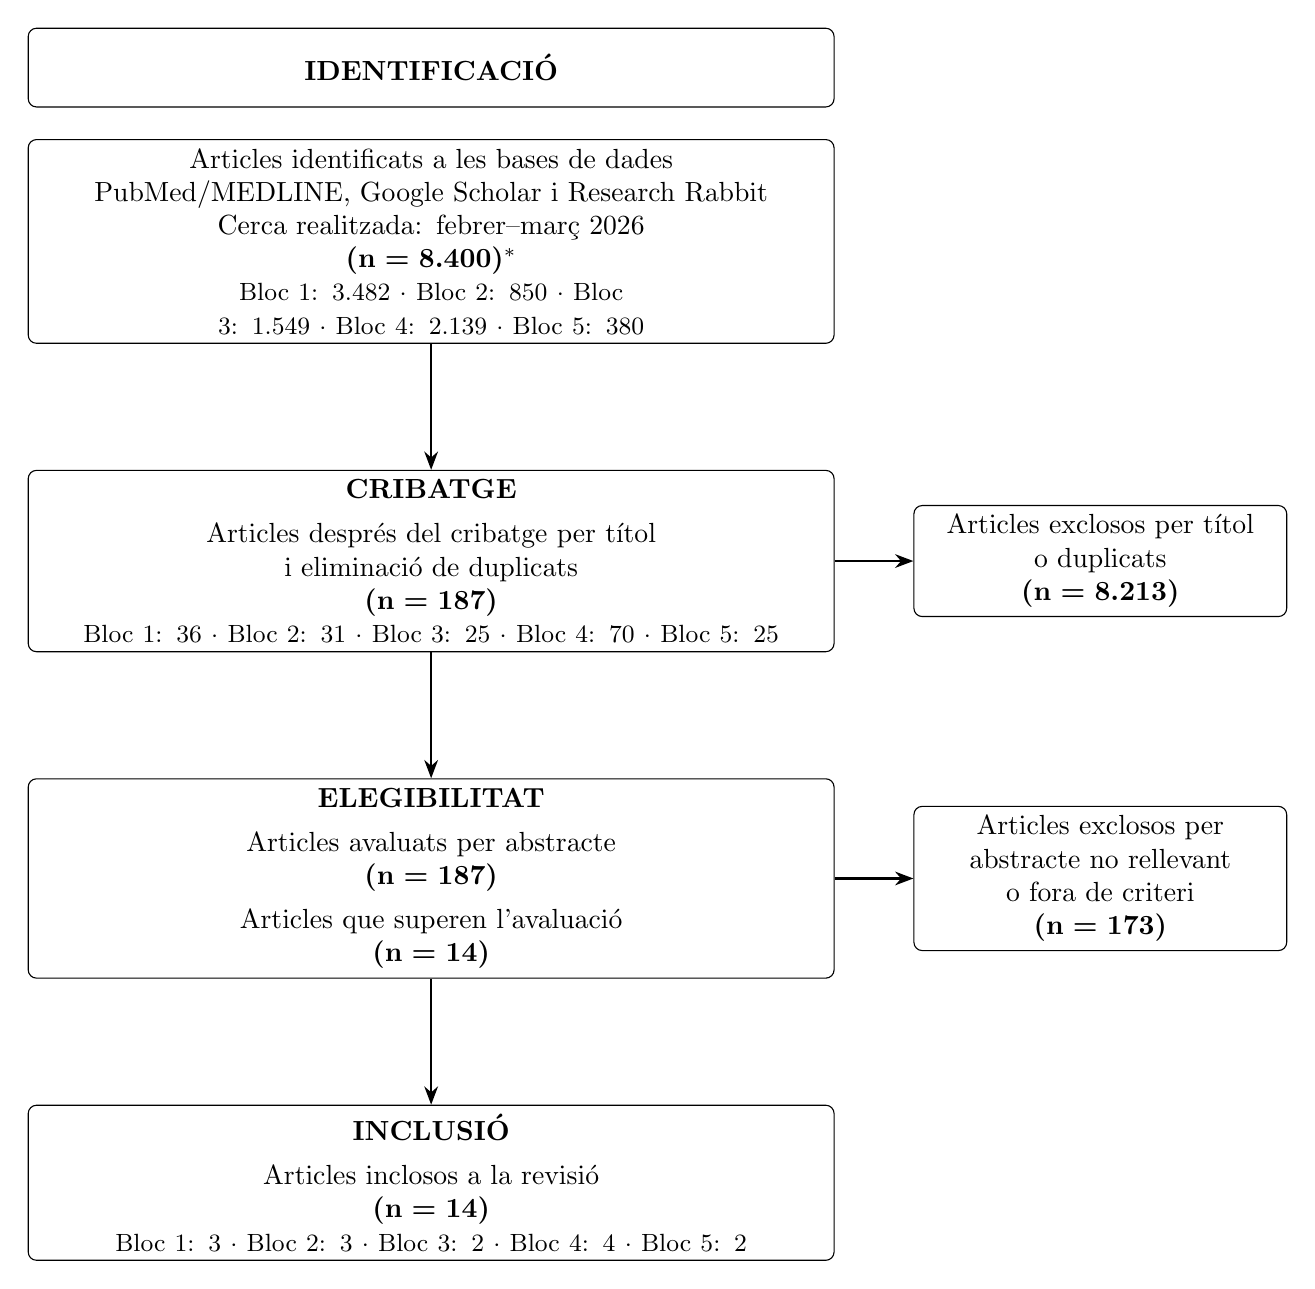
\begin{tikzpicture}[
    box/.style={rectangle, draw=black, rounded corners=3pt, 
                text width=10cm, minimum height=1cm, 
                align=center, fill=white},
    smallbox/.style={rectangle, draw=black, rounded corners=3pt,
                text width=4.5cm, minimum height=1cm,
                align=center, fill=white},
    arrow/.style={-{Stealth}, thick},
    node distance=1.2cm
]

%% IDENTIFICACIÓ
\node[box] (id_title) {
    \textbf{IDENTIFICACIÓ}
};

\node[box, below=0.4cm of id_title] (id_box) {
    Articles identificats a les bases de dades\\
    PubMed/MEDLINE, Google Scholar i Research Rabbit\\
    Cerca realitzada: febrer--març 2026\\
    \textbf{(n = 8.400)}$^{*}$\\
    \small Bloc 1: 3.482 $\cdot$ Bloc 2: 850 $\cdot$ Bloc 3: 1.549 
    $\cdot$ Bloc 4: 2.139 $\cdot$ Bloc 5: 380
};

%% CRIBATGE
\node[box, below=1.6cm of id_box] (crib_box) {
    \textbf{CRIBATGE}\\[4pt]
    Articles després del cribatge per títol\\
    i eliminació de duplicats\\
    \textbf{(n = 187)}\\
    \small Bloc 1: 36 $\cdot$ Bloc 2: 31 $\cdot$ Bloc 3: 25 
    $\cdot$ Bloc 4: 70 $\cdot$ Bloc 5: 25
};

\node[smallbox, right=1cm of crib_box] (excl1) {
    Articles exclosos per títol\\
    o duplicats\\
    \textbf{(n = 8.213)}
};

\draw[arrow] (id_box) -- (crib_box);
\draw[arrow] (crib_box.east) -- (excl1.west);

%% ELEGIBILITAT
\node[box, below=1.6cm of crib_box] (eleg_box) {
    \textbf{ELEGIBILITAT}\\[4pt]
    Articles avaluats per abstracte\\
    \textbf{(n = 187)}\\[4pt]
    Articles que superen l'avaluació\\
    \textbf{(n = 14)}
};

\node[smallbox, right=1cm of eleg_box] (excl2) {
    Articles exclosos per\\
    abstracte no rellevant\\
    o fora de criteri\\
    \textbf{(n = 173)}
};

\draw[arrow] (crib_box) -- (eleg_box);
\draw[arrow] (eleg_box.east) -- (excl2.west);

%% INCLUSIÓ
\node[box, below=1.6cm of eleg_box] (incl_box) {
    \textbf{INCLUSIÓ}\\[4pt]
    Articles inclosos a la revisió\\
    \textbf{(n = 14)}\\
    \small Bloc 1: 3 $\cdot$ Bloc 2: 3 $\cdot$ Bloc 3: 2 
    $\cdot$ Bloc 4: 4 $\cdot$ Bloc 5: 2
};

\draw[arrow] (eleg_box) -- (incl_box);

\end{tikzpicture}
\caption{Diagrama de flux PRISMA del procés de selecció bibliogràfica. Per als blocs amb volum elevat de resultats, la selecció s'ha aplicat sobre els articles de major impacte i rellevància temàtica seguint una estratègia de saturació temàtica. $^{*}$Els resultats dels blocs 1 (n\,=\,3.482), 3 (n\,=\,1.549) i 4 (n\,=\,2.139) corresponen als volums documentats en les revisions sistemàtiques de referència consultades. La selecció final s'ha aplicat seguint criteris de rellevància temàtica i impacte científic.}
\label{fig:prisma}
\end{figure}

\section{Síntesi de la literatura per blocs temàtics}

\subsection{Bloc 1: Càrrega administrativa en sistemes sanitaris}

La sobrecàrrega administrativa dels professionals sanitaris constitueix un problema estructural ben documentat en la literatura científica. L'estudi seminal de Sinsky et al.~\cite{sinsky2016allocation}, realitzat mitjançant observació directa de 57 metges de quatre especialitats als Estats Units, va evidenciar que els professionals dediquen únicament el 27\% de la seva jornada laboral a l'atenció directa al pacient, mentre que el 49,2\% del temps s'inverteix en tasques documentals i de gestió de l'historial electrònic. A més, els professionals dediquen entre una i dues hores addicionals cada nit, fora de l'horari laboral, a completar tasques documentals pendents. Aquestes dades posen de manifest una paradoxa estructural del sistema sanitari modern: el professional que hauria de tenir el pacient com a centre de la seva activitat destina gairebé la meitat del seu temps a tasques de naturalesa administrativa.

Aquesta problemàtica no és exclusiva del context nord-americà. De Hoop i Neumuth~\cite{dehoop2021ehr}, en un estudi observacional directe realitzat en un gran centre universitari alemany amb 19 metges de sis departaments, van constatar que el 37,1\% del temps observat es dedicava a interaccions amb l'historial electrònic ---un 20,5\% en tasques de documentació, un 9,0\% en cerca d'informació i un 7,7\% en lectura--- mentre que únicament el 28,0\% es destinava a la interacció directa amb els pacients. Els professionals van identificar com a principals fonts de descontentament l'alta càrrega documental repetitiva, la dispersió de la informació del pacient entre diferents sistemes i l'impacte d'aquests problemes en la qualitat de la interacció assistencial. Aquests resultats, obtinguts en un context europeu continental, reforcen la dimensió estructural i transversal del problema i suggereixen la seva aplicabilitat directa a sistemes sanitaris similars com el sistema sanitari públic espanyol.

Aquesta problemàtica no ha millorat amb el pas del temps. La revisió sistemàtica de Murad et al.~\cite{murad2024documentation}, que analitza 135 estudis publicats entre 2010 i 2023, confirma que la sobrecàrrega documental segueix sent un dels principals factors associats a l'esgotament professional (\textit{burnout}) en l'àmbit sanitari, amb un impacte negatiu mesurable en la satisfacció laboral, l'equilibri vida-feina i, en última instància, en la qualitat de l'atenció al pacient. La revisió identifica onze categories de mesura de la sobrecàrrega documental, des del temps total dedicat a l'historial electrònic fins a la gestió de bústies d'entrada, derivacions i tasques administratives de facturació i assegurances, reflectint la complexitat i la multicausalitat del problema.

En conjunt, l'evidència disponible confirma que la sobrecàrrega documental és un problema estructural, persistent i transversal als sistemes sanitaris occidentals, amb un impacte directe en la qualitat de l'atenció al pacient i el benestar dels professionals. Aquesta realitat justifica la necessitat de solucions tecnològiques que redueixin de forma significativa la càrrega documental sense comprometre la qualitat ni la traçabilitat de la documentació clínica generada.

\subsection{Bloc 2: Models de llenguatge aplicats a salut}

L'aplicació dels models de llenguatge en l'àmbit sanitari ha experimentat un creixement exponencial en els darrers anys, convertint-se en una de les línies de recerca més actives de la intersecció entre la intel·ligència artificial i la medicina. La revisió sistemàtica de Bedi et al.~\cite{bedi2025llm}, que analitza 519 estudis publicats entre 2022 i 2024, ofereix una panoràmica exhaustiva de l'estat actual d'aquesta recerca. Els resultats revelen que les tasques més estudiades són l'avaluació de coneixement mèdic (44,5\% dels estudis) i el suport diagnòstic (19,5\%), mentre que les tasques de documentació clínica i gestió administrativa ---com l'assignació de codis de facturació (0,2\%) o la redacció de prescripcions (0,2\%)--- representen una fracció mínima de la recerca existent. A més, el 95,4\% dels estudis utilitza la precisió com a única dimensió d'avaluació i només el 5\% empra dades reals de pacients, cosa que limita la validesa externa dels resultats en contextos clínics reals. Aquests buits de recerca identifiquen i justifiquen directament l'espai que el present projecte pretén explorar.

En el context específic dels sistemes sanitaris públics, on les infraestructures computacionals disponibles sovint no disposen de maquinari especialitzat i on els requisits de privacitat de les dades clíniques limiten l'ús de serveis externs al núvol, els models de gran escala presenten limitacions pràctiques significatives. És en aquest context on els \textbf{models de llenguatge de menor mida} (\textit{Small Language Models}, SLMs) emergeixen com l'alternativa més adequada. Garg et al.~\cite{garg2025slm} presenten una revisió exhaustiva sobre l'ús de SLMs en entorns sanitaris, identificant tres avantatges fonamentals per al context que ens ocupa: en primer lloc, els SLMs redueixen el consum energètic entre 10 i 100 vegades respecte als LLMs de gran escala mitjançant tècniques d'optimització i compressió de models; en segon lloc, la seva mida reduïda permet el desplegament local sense necessitat de transmetre dades a servidors externs, garantint la privacitat de les dades clíniques dels pacients; en tercer lloc, ofereixen latències d'inferència molt inferiors, essencials en escenaris assistencials que requereixen respostes en temps real.

Un aspecte crític en la selecció del model és si la reducció de mida implica una pèrdua inacceptable de qualitat clínica. L'estudi de Kocaman et al.~\cite{kocaman2025clever}, que compara GPT-4o amb SLMs especialitzats en salut de 8B i 70B paràmetres en tres tasques clíniques ---resum de text clínic, extracció d'informació i resposta a preguntes biomèdiques--- aporta evidència empírica rellevant en aquest sentit. Els resultats mostren que els metges participants van preferir els SLMs especialitzats sobre GPT-4o entre un 45\% i un 92\% més sovint en les dimensions de factualitat, rellevància clínica i concisió. Aquests resultats suggereixen que els SLMs entrenats específicament en domini clínic no només són computacionalment viables sinó que poden superar els LLMs generals en tasques de documentació assistencial, reforçant la seva idoneïtat com a component base del sistema proposat en aquest projecte.

En conjunt, l'evidència disponible justifica l'elecció dels SLMs com a tecnologia base del sistema proposat, oferint un equilibri òptim entre capacitat de comprensió i generació de text clínic, eficiència computacional i viabilitat de desplegament en infraestructures sanitàries públiques sense maquinari especialitzat.

\subsection{Bloc 3: Ontologies semàntiques mèdiques}

El coneixement mèdic es caracteritza per una complexitat terminològica excepcional: un mateix concepte clínic pot expressar-se de múltiples formes ---noms científics, acrònims, denominacions col·loquials--- i les relacions entre conceptes són sovint jeràrquiques, causals o funcionals. En aquest context, les ontologies semàntiques mèdiques constitueixen una eina fonamental per estructurar, representar i intercanviar coneixement clínic de forma precisa i interoperable. Parsanasab et al.~\cite{parsanasab2025ontologies} revisen l'ús d'ontologies en el desenvolupament de sistemes d'intel·ligència artificial en salut, concloent que les ontologies milloren la precisió dels resultats dels sistemes d'IA, donen suport a la presa de decisions mèdiques i habiliten l'intercanvi semàntic de dades diverses i heterogènies. Els autors destaquen que les ontologies són essencials per al desenvolupament de sistemes de suport a la decisió clínica i per fomentar interaccions intel·ligents entre pacients i sistemes sanitaris, subratllant el seu paper com a capa de coneixement estructurat que complementa i enriqueix les capacitats dels models d'intel·ligència artificial.

Des d'un punt de vista pràctic, l'accés i la reutilització d'ontologies biomèdiques és possible gràcies a infraestructures obertes com BioPortal, documentada per Vendetti et al.~\cite{vendetti2025bioportal}. BioPortal és el repositori més complet del món d'ontologies biomèdiques, amb 1.549 ontologies públiques accessibles, entre les quals es troben els estàndards més rellevants per al present projecte: \textbf{SNOMED~CT} (\textit{Systematized Nomenclature of Medicine -- Clinical Terms}), el sistema de codificació clínica més complet i utilitzat internacionalment, i \textbf{LOINC} (\textit{Logical Observation Identifiers Names and Codes}), l'estàndard universal per a la identificació d'observacions i mesures clíniques com resultats de laboratori i signes vitals. L'accessibilitat programàtica d'aquestes ontologies mitjançant una API REST facilita la seva integració en pipelines de processament automatitzat, com la que el present projecte proposa implementar.

La combinació d'ontologies semàntiques amb sistemes d'IA generativa presenta avantatges específics en el context de la documentació clínica. En primer lloc, permeten resoldre ambigüitats terminològiques ---garantint que el sistema reconegui que \textit{insuficiència cardíaca congestiva}, \textit{ICC} i el codi SNOMED~CT \textit{42343007} fan referència al mateix concepte clínic--- i produir documentació amb terminologia precisa i consistent. En segon lloc, les relacions jeràrquiques i semàntiques entre conceptes permeten al sistema inferir informació rellevant més enllà de les coincidències textuals literals, millorant la qualitat de la recuperació d'informació en arquitectures RAG. Finalment, la traçabilitat dels codis ontològics en els documents generats facilita l'auditoria clínica i el compliment dels requisits legals de documentació en sistemes sanitaris públics regulats.

En conjunt, les ontologies semàntiques mèdiques no constitueixen un element accessori del sistema proposat, sinó un component estructural que garanteix la precisió terminològica, la coherència semàntica i la traçabilitat clínica de la documentació generada ---tres requisits crítics identificats en la descripció de la proposta d'aquest projecte.

\subsection{Bloc 4: Arquitectures RAG en entorns sanitaris}

Les arquitectures de \textit{Retrieval-Augmented Generation} (RAG) sorgeixen com a resposta a les limitacions fonamentals dels models de llenguatge aplicats en dominis especialitzats com el sanitari. Lewis et al.~\cite{lewis2020retrieval}, en el treball seminal que va establir les bases d'aquesta arquitectura, demostren que els models de llenguatge pateixen tres limitacions crítiques en contextos d'alt rigor: la generació de contingut al·lucinat no fonamentat en fonts verificables, l'obsolescència del coneixement incorporat durant l'entrenament i la manca de transparència sobre l'origen de la informació generada. RAG aborda aquestes limitacions exposant el model a fonts de coneixement externes i verificades en el moment de la generació, de manera que cada resposta es fonamenta en documents reals recuperats dinàmicament ---una propietat especialment crítica en entorns sanitaris on la traçabilitat documental és un imperatiu legal i clínic.

L'aplicació de RAG en l'àmbit sanitari ha estat objecte d'una revisió sistemàtica exhaustiva per part d'Amugongo et al.~\cite{amugongo2025rag}, que analitza 70 estudis publicats entre 2020 i 2025 seleccionats d'un corpus inicial de 2.139 articles. Els autors identifiquen tres generacions d'arquitectures RAG en salut: \textit{Naive RAG}, que implementa una recuperació vectorial simple; \textit{Advanced RAG}, que incorpora estratègies de reranking i filtratge; i \textit{Modular RAG}, que permet la composició flexible de components especialitzats. La revisió constata que els models propietaris GPT-3.5/4 predominen en els estudis actuals, i identifica com a buits rellevants la manca de frameworks d'avaluació estandarditzats i la insuficient consideració de les implicacions ètiques i de privacitat en el desplegament clínic --- buits que el present projecte aborda mitjançant l'ús de SLMs locals i mètriques d'avaluació específiques del domini.

L'evidència quantitativa sobre l'impacte de RAG en la qualitat dels LLMs en biomedicina és sòlida. Liu, McCoy i Wright~\cite{liu2025rag}, en una metaanàlisi de 20 estudis comparatius, reporten un \textit{pooled effect size} d'1,35 (IC 95\%: 1,19--1,53; p\,=\,0,001), indicant que les arquitectures RAG milloren significativament el rendiment dels models base en tasques biomèdiques. A més, els autors proposen el framework \textbf{GUIDE-RAG}, que estructura la implementació clínica en tres etapes: pre-recuperació ---definició de l'estratègia de cerca i preparació del corpus---, recuperació ---selecció i reranking dels documents rellevants--- i post-recuperació ---generació i validació de la resposta. Aquest framework ofereix una guia metodològica directament aplicable al disseny del sistema proposat en aquest projecte.

Finalment, la combinació específica de RAG amb ontologies semàntiques representa una línia emergent de recerca de gran rellevància per al present projecte. Feng et al.~\cite{feng2025ontologyrag} demostren, en el context del mapatge de codis biomèdics, que la incorporació de grafs d'ontologia en arquitectures RAG millora tant la precisió com l'eficiència del sistema respecte a enfocaments RAG purament textuals. Els grafs ontològics permeten establir relacions semàntiques entre conceptes que la cerca vectorial convencional no és capaç de capturar, millorant la qualitat de la recuperació en consultes amb alta càrrega terminològica clínica ---exactament el tipus de consultes que el sistema proposat haurà de gestionar en la generació d'informes d'alta i derivacions.

En conjunt, l'evidència disponible demostra que les arquitectures RAG constitueixen la solució tècnica més adequada per abordar les limitacions dels models de llenguatge en entorns sanitaris regulats, garantint la traçabilitat, la precisió terminològica i la coherència clínica de les respostes generades. La combinació d'aquesta arquitectura amb ontologies semàntiques mèdiques representa una línia d'investigació emergent amb un potencial significatiu, especialment en tasques de documentació clínica on la precisió terminològica i l'alineació amb estàndards oficials són imperatius no negociables. Aquests fonaments teòrics i empírics, juntament amb els reptes d'eficiència computacional, privacitat de dades i qualitat de la documentació generada identificats en la literatura revisada, justifiquen la necessitat d'aprofundir en la integració d'ontologies semàntiques en arquitectures RAG aplicades a la documentació clínica assistida.

\subsection{Bloc 5: Generació automàtica de documentació clínica}

La generació automàtica de documentació clínica mitjançant models de llenguatge representa l'aplicació pràctica més directa de les tecnologies revisades en els blocs anteriors. Els informes d'alta hospitalària constitueixen un dels processos documentals de major volum i impacte en els sistemes sanitaris públics, i la seva generació manual és un procés que consumeix un temps significatiu dels professionals sanitaris, amb una qualitat variable en funció de la càrrega assistencial i l'experiència del redactor. Chua et al.~\cite{chua2024discharge} presenten un estudi pilot realitzat en un hospital de Singapur on el sistema RUSSELL GPT, basat en un LLM personalitzat, va ser desplegat en un entorn clínic real per a la generació assistida d'informes d'alta. Els resultats mostren una reducció del temps de redacció de 10 a 6 minuts per informe, amb una projecció d'estalvi de 1.285 hores-home anuals per als 19.300 informes d'alta completats el 2023. Els autors subratllen que la càrrega de redacció d'informes d'alta recau habitualment en els metges residents, i que la qualitat dels documents és variable en funció de la seniority del professional i el seu grau d'implicació durant l'ingrés, cosa que presenta riscos potencials de seguretat en la transició de l'hospital a l'atenció primària. Aquest estudi proporciona evidència directa de la viabilitat i l'impacte pràctic de la generació assistida d'informes clínics en un entorn hospitalari real, validant el cas d'ús principal del present projecte.

Des d'un punt de vista metodològic, Ellershaw et al.~\cite{ellershaw2024discharge} proposen un enfocament basat en \textit{few-shot prompting} ---una tècnica que proporciona al model uns quants exemples del tipus de resposta esperada directament a l'entrada, sense necessitat d'un procés d'entrenament específic--- guiat per les guies clíniques del Royal College of Physicians de Londres per a la generació automàtica d'informes d'alta hospitalària. A diferència dels enfocaments supervisats anteriors, el seu mètode no requereix un gran conjunt de dades d'entrenament etiquetades, accepta notes mèdiques completes com a input i es guia explícitament per les millors pràctiques clíniques establertes. El sistema, implementat amb GPT-4-turbo i avaluat per 10 clínics sobre 53 informes generats a partir de dades del corpus MIMIC-III, va obtenir una precisió micro de 0,81. Aquest estudi valida un principi metodològic fonamental que el present projecte comparteix: fonamentar la generació de documentació clínica en fonts oficials verificades garanteix una major adherència clínica i qualitat documental. No obstant això, l'absència d'una capa de coneixement ontològic en aquest enfocament deixa sense resoldre el repte de la coherència terminològica ---un aspecte crític en entorns sanitaris regulats on un mateix concepte clínic pot expressar-se de múltiples formes al llarg d'un mateix document.

La limitació identificada en l'estudi d'Ellershaw et al. és extensible al treball de Chua et al., on el sistema RUSSELL GPT es basa en un LLM personalitzat sense integració ontològica explícita. En ambdós casos, l'absència d'una capa de coneixement estructurat pot resultar en inconsistències terminològiques i en una traçabilitat limitada dels conceptes clínics presents en els documents generats ---aspectes especialment crítics en sistemes sanitaris públics regulats, on la precisió terminològica i l'audibilitat dels documents clínics constitueixen requisits legals i assistencials no negociables. Aquesta limitació comuna als treballs existents defineix el buit específic que el present projecte pretén abordar mitjançant la incorporació d'ontologies semàntiques mèdiques com a capa de coneixement estructurat en l'arquitectura RAG proposada.

En conjunt, els treballs revisats demostren la viabilitat tècnica i el valor pràctic de la generació automàtica de documentació clínica en entorns hospitalaris reals, amb impactes mesurables en la reducció del temps de redacció i la millora de la qualitat documental. Al mateix temps, la manca d'integració ontològica en els sistemes existents identifica un buit específic en la recerca actual que el present projecte aborda, situant la proposta en la frontera del coneixement en aquest domini i justificant la seva rellevància científica i pràctica.



\chapter{Disseny i implementació}

Aquest capítol descriu el disseny i la implementació del sistema \textit{Healthcare RAG-SLM}, des de les especificacions funcionals i no funcionals fins a l'arquitectura tècnica concreta, l'\textit{stack} de desenvolupament i les decisions de disseny preses durant el desenvolupament. S'estructura de manera progressiva, des de la definició dels requisits del sistema fins als detalls d'implementació de cada cas d'ús, incloent la justificació empírica de la selecció del model de llenguatge a partir de mesures comparatives reals.

\section{Especificacions de la solució}

En qualsevol projecte d'enginyeria de programari, la definició formal de les especificacions constitueix el primer pas fonamental del procés de disseny, ja que estableix el contracte explícit entre els objectius del projecte i la seva materialització tècnica. Situar les especificacions com a primera secció del capítol de disseny i implementació respon a una lògica metodològica precisa: abans de descriure \textit{com} s'ha construït el sistema (arquitectura, tecnologies, implementació), cal definir amb rigor \textit{què} ha de fer i \textit{sota quines restriccions} ha d'operar. Aquesta seqüència garanteix que cada decisió de disseny posterior ---des de l'elecció del model de llenguatge fins a l'arquitectura d'infraestructura--- pot ser justificada i traçada cap a un requisit concret, evitant implementacions \textit{ad hoc} sense fonament en les necessitats reals del sistema.

En el context d'aquest projecte, les especificacions compleixen una triple funció. En primer lloc, actuen com a \textbf{pont entre els objectius} formulats al capítol introductori i les decisions tècniques preses durant el desenvolupament: cada objectiu secundari es descomposa en un o diversos requisits verificables que guien la implementació. En segon lloc, les especificacions proporcionen els \textbf{criteris d'avaluació} objectius contra els quals es mesurarà l'èxit del sistema al capítol de resultats: un requisit funcional no satisfet o un requisit no funcional incomplert constitueix una deficiència objectiva i mesurable. En tercer lloc, en un domini altament regulat com el sanitari, les especificacions estableixen les \textbf{condicions de seguretat i conformitat normativa} ---privacitat de dades, supervisió humana, traçabilitat--- que el sistema ha de respectar per ser considerat viable en un entorn de producció real.

Les especificacions s'organitzen en dos grups complementaris: \textbf{requisits funcionals} (RF) i \textbf{requisits no funcionals} (RNF). Aquesta distinció, establerta en l'enginyeria de requisits i recollida en estàndards com l'ISO/IEC~25010, separa les capacitats operatives del sistema de les seves propietats de qualitat.

Els \textbf{requisits funcionals} defineixen \textit{què} ha de fer el sistema, és a dir, les funcionalitats concretes que ha d'oferir als seus usuaris. En el nostre cas, inclouen les capacitats de generació documental per a cada tipologia clínica, la recuperació contextual de protocols, la codificació ontològica automàtica, la detecció d'especialitat i la interacció amb l'usuari. Cada requisit funcional descriu un comportament observable i verificable del sistema davant d'una entrada determinada: donada una petició amb dades clíniques concretes, el sistema ha de produir una sortida amb característiques especificades.

Els \textbf{requisits no funcionals}, en canvi, delimiten \textit{com} ha de funcionar el sistema en termes de qualitat, rendiment i restriccions operatives. No descriuen funcionalitats noves, sinó atributs de qualitat que condicionen l'experiència d'ús i la viabilitat del desplegament. En un sistema sanitari, aquests requisits adquireixen una importància \textit{crítica}: un sistema que genera informes clínics correctes però que requereix 5~minuts per document, que consumeix 32~GB de RAM o que transmet dades de pacients a servidors externs seria tècnicament funcional però operativament inacceptable en el context d'un centre sanitari públic. Per tant, els requisits no funcionals defineixen l'espai de solucions viables dins del qual el sistema ha d'operar, i la seva violació pot ser tant o més greu que la d'un requisit funcional.

\subsection{Requisits funcionals}

Els requisits funcionals del sistema s'han derivat directament dels objectius del projecte i dels tres casos d'ús clínics prioritzats a la fase de definició. Cada requisit es presenta amb una descripció detallada que inclou les condicions d'acceptació implícites i la justificació de la seva necessitat en el context del projecte.

\begin{itemize}
    \item \textbf{RF-1. Generació d'informes d'alta hospitalària:} El sistema ha de generar esborranys d'informes d'alta a partir de les dades clíniques d'entrada del pacient (motiu d'ingrés, diagnòstic, medicació, procediments), produint un document estructurat en \textbf{nou seccions obligatòries}: dades del pacient, motiu d'ingrés, diagnòstic principal, diagnòstics secundaris, procediments realitzats, tractament i medicació, evolució clínica, recomanacions de seguiment i contraindicacions. Aquest requisit respon directament a l'objectiu principal del projecte i al cas d'ús de major impacte estimat: la literatura reporta un temps mitjà de redacció de 10~minuts per informe d'alta~\cite{chua2024discharge}, representant milers d'hores anuals de feina documental en qualsevol sistema sanitari públic de mida mitjana. L'estructura de nou seccions s'ha definit a partir de l'anàlisi dels estàndards documentals dels serveis de salut de referència i garanteix la cobertura de tots els elements clínicament rellevants per a la continuïtat assistencial.

    \item \textbf{RF-2. Generació d'informes de derivació:} El sistema ha de generar documents de derivació a un especialista o servei concret, incloent dades del pacient, especialitat destí, motiu clínic, antecedents rellevants, exploracions realitzades, tractament actual i informació addicional per a l'especialista. El document pot incloure opcionalment una suggerència de classificació d'urgència (normal, preferent, urgent) basada en el context clínic, tot i que la decisió final sobre la prioritat recau sempre en el professional sanitari. L'estructura s'ha definit seguint els protocols de derivació del sistema sanitari públic, garantint la inclusió de tota la informació necessària per a la continuïtat assistencial.

    \item \textbf{RF-3. Generació de resums clínics previs a consulta:} El sistema ha de produir una síntesi automatitzada i concisa (objectiu de 150--200~paraules) de la informació clínica rellevant del pacient ---símptomes actuals, medicació habitual amb codificació ATC, antecedents, especialitat--- per facilitar la preparació del professional sanitari abans de la visita. A diferència dels altres dos casos d'ús, aquest resum incorpora la \textbf{detecció automàtica d'interaccions medicamentoses} i la generació d'\textbf{alertes clíniques} (interaccions fàrmac-malaltia, fàrmac-fàrmac i condició-condició), classificades per severitat (crítica, moderada, baixa), atès que el seu objectiu és precisament preparar el professional per a la consulta amb informació accionable i rellevant per a la seguretat del pacient.

    \item \textbf{RF-4. Recuperació contextual de protocols:} El sistema ha de recuperar dinàmicament els protocols i guies clíniques rellevants per a cada cas concret mitjançant cerca semàntica vectorial sobre un corpus indexat, fonamentant la generació en fonts oficials verificades. Cada protocol recuperat ha d'incloure un \textit{score} de similitud semàntica que permeti al sistema i a l'usuari avaluar la rellevància de la font. El nombre de protocols recuperats per defecte s'ha establert en cinc (\texttt{RETRIEVAL\_TOP\_K=10}, amb \textit{reranking} a 5), amb un llindar mínim de similitud de 0,5 per garantir la pertinença dels resultats. Aquest requisit és essencial per a l'enfocament RAG del sistema: la generació no es basa exclusivament en el coneixement intern del model de llenguatge, sinó que es fonamenta en fonts clíniques verificades i actualitzables, reduint el risc d'al·lucinacions i garantint l'alineació amb els protocols vigents.

    \item \textbf{RF-5. Detecció automàtica d'especialitat:} El sistema ha de detectar automàticament l'especialitat clínica del cas a partir del context del pacient (motiu d'ingrés, diagnòstics, símptomes) mitjançant un diccionari de \textit{keywords} clíniques, amb cobertura de com a mínim onze especialitats principals: cardiologia, neurologia, endocrinologia, dermatologia, gastroenterologia, reumatologia, pneumologia, nefrologia, hematologia, cirurgia general i medicina interna. Aquesta detecció s'utilitza com a \textbf{filtre durant la recuperació} de protocols, permetent restringir la cerca als documents rellevants per a l'especialitat del cas i millorant la precisió de la informació recuperada. En el cas de derivació, la detecció d'especialitat permet també la \textbf{validació de coherència} entre el motiu de derivació i l'especialitat destí, generant alertes quan es detecten inconsistències.

    \item \textbf{RF-6. Codificació ontològica automàtica:} El sistema ha d'enllaçar les entitats clíniques detectades al document generat amb els codis ontològics corresponents de les principals terminologies mèdiques internacionals: \textbf{SNOMED~CT} per a diagnòstics i procediments clínics (terminologia clínica de referència amb més de 350.000~conceptes), \textbf{ICD-10} per a la classificació internacional de malalties (estàndard de codificació per a facturació i estadístiques sanitàries), \textbf{ATC} (\textit{Anatomical Therapeutic Chemical Classification}) per a la classificació de medicaments, i opcionalment \textbf{MeSH} (\textit{Medical Subject Headings}) per a descriptors bibliogràfics. Cada codi assignat ha d'incloure un nivell de confiança numèric (entre 0 i 1) i la font de la codificació (cerca semàntica local o \textit{fallback} a BioPortal). La codificació ontològica constitueix l'aportació diferencial del sistema respecte a enfocaments RAG purament textuals i és fonamental per a la \textbf{interoperabilitat} amb sistemes d'informació sanitària existents (HIS, HCE).

    \item \textbf{RF-7. Traçabilitat completa:} Cada document generat ha d'incloure un conjunt complet de metadades de traçabilitat: les referències a les fonts utilitzades (protocols recuperats amb \textit{score} de similitud), els codis ontològics de tots els conceptes clínics mencionats amb el seu nivell de confiança i font de codificació, el temps total de generació desglossat per component del pipeline, l'especialitat detectada, el nombre de consultes externes realitzades (per exemple, \textit{fallback} a BioPortal) i l'estat de validació del document. Aquesta traçabilitat permet al professional sanitari verificar les fonts del document generat i constitueix un requisit imprescindible per al desplegament en entorns clínics regulats, on l'auditabilitat de les decisions assistencials és una obligació legal i on la responsabilitat final recau sempre en el professional.

    \item \textbf{RF-8. Suport multilingüe:} El sistema ha de suportar la generació de documents en català, castellà i anglès, atenent les necessitats lingüístiques del context sanitari objectiu. El model d'\textit{embeddings} seleccionat ha de proporcionar suport natiu per a les tres llengües, permetent la recuperació semàntica \textit{cross-lingual} ---per exemple, recuperar protocols en castellà a partir d'una consulta en català. El model de llenguatge ha de ser capaç de generar text coherent i terminològicament precís en les tres llengües sense degradació significativa de la qualitat. La necessitat multilingüe respon al fet que els protocols oficials sovint estan redactats en castellà o anglès, mentre que la interacció amb el sistema pot ser en qualsevol de les tres llengües.

    \item \textbf{RF-9. Interfície d'usuari:} El sistema ha de disposar d'una interfície web funcional que permeti al professional sanitari seleccionar pacients de mostra, escollir la tipologia documental desitjada (informe d'alta, derivació o resum clínic), visualitzar el document generat amb format professional i llegible, consultar els codis ontològics assignats amb el seu nivell de confiança, i accedir a les fonts de traçabilitat (protocols recuperats). La interfície ha de proporcionar retroalimentació visual durant el procés de generació, temps de càrrega inicial inferiors a 2~segons i una experiència d'ús adaptada al context sanitari, amb un disseny \textit{responsive} que permeti l'ús en diferents dispositius.
\end{itemize}

\subsection{Requisits no funcionals}

Els requisits no funcionals defineixen les propietats de qualitat que condicionen la viabilitat del sistema en un entorn sanitari real. S'han derivat de l'anàlisi de les restriccions operatives dels sistemes sanitaris públics, dels requisits legals i normatius aplicables (RGPD, LOPD, normativa sanitària) i de les bones pràctiques d'enginyeria de programari per a sistemes crítics.

\begin{itemize}
    \item \textbf{RNF-1. Eficiència computacional:} El sistema ha de poder operar en infraestructures sanitàries estàndard sense maquinari especialitzat ---específicament, en estacions de treball amb CPU sense GPU dedicada---, amb un consum màxim de RAM de 16~GB i ser viable també en dispositius amb 8~GB de memòria. Aquesta restricció reflecteix la realitat de les infraestructures TIC dels sistemes sanitaris públics, on els equips disponibles rarament disposen d'acceleradors gràfics dedicats i on la memòria disponible ha de ser compartida amb altres aplicacions clíniques (historial electrònic, sistemes de prescripció, eines de diagnòstic per imatge). El model de llenguatge, com a component més intensiu computacionalment del pipeline, ha de poder executar-se en mode CPU amb un consum de RAM inferior a 4~GB per garantir la coexistència amb la resta d'aplicacions.

    \item \textbf{RNF-2. Latència objectiu:} La generació d'un document complet ---des de la recepció de la petició fins a la construcció de la resposta JSON amb totes les metadades de traçabilitat--- ha d'oferir un temps de resposta inferior a 30~segons en condicions de càrrega normal (un sol usuari concurrent). Aquest objectiu s'ha establert a partir de la literatura sobre usabilitat en entorns sanitaris, que indica que els professionals consideren acceptable una espera de fins a 30~segons per a la generació d'un document que manualment requeriria entre 6 i 10~minuts. Temps superiors a 60~segons provoquen una percepció d'ineficiència que compromet l'adopció del sistema. La interfície ha de proporcionar retroalimentació visual clara durant el procés de generació (indicador de progrés, estat del procés) per evitar que l'usuari percebi el sistema com a no responsiu. L'objectiu implícit és que la latència total del pipeline no estigui dominada per cap component individual en una proporció superior al 80\%.

    \item \textbf{RNF-3. Privacitat i sobirania de les dades:} Tot el processament s'ha de realitzar localment, sense transmissió de dades clíniques a serveis externs al núvol, garantint el compliment del Reglament General de Protecció de Dades (RGPD), la Llei Orgànica de Protecció de Dades (LOPD) i la normativa sanitària aplicable. El sistema ha de poder funcionar completament \textit{offline} després de la fase d'ingesta inicial, ja que les dades dels pacients mai surten de l'entorn local. L'única comunicació externa permesa és la consulta a BioPortal durant la fase de codificació ontològica, que transmet únicament termes clínics genèrics (no dades identificatives de pacients) i que, a més, funciona com a mecanisme de \textit{fallback} activat en menys del 10\% dels casos. Aquesta decisió arquitectònica ---inferència local amb Ollama, emmagatzematge local amb Qdrant--- és fonamental en el context sanitari, on la protecció de la informació clínica no és només un requisit tècnic sinó un imperatiu legal i ètic.

    \item \textbf{RNF-4. Modularitat i extensibilitat:} L'arquitectura ha de permetre la substitució independent dels seus components principals ---model de llenguatge, base de dades vectorial, model d'\textit{embeddings}, serveis d'ontologies--- sense requerir modificacions en la resta del sistema. Aquesta modularitat facilita l'evolució tecnològica (per exemple, la substitució del model Llama~3.2 per una versió futura més potent), l'adaptació a entorns diferents (per exemple, substituir Qdrant per un altre magatzem vectorial disponible a la infraestructura objectiu) i el manteniment a llarg termini. L'arquitectura ha de seguir el principi d'inversió de dependències, amb interfícies ben definides entre els mòduls, de manera que els components d'alt nivell (lògica de negoci) no depenguin directament dels components de baix nivell (infraestructura), sinó d'abstraccions compartides.

    \item \textbf{RNF-5. Reproductibilitat:} El sistema ha de ser desplegable de manera reproduïble mitjançant contenidors Docker i configuració declarativa (Docker Compose), amb totes les dependències, versions i configuracions documentades explícitament. Un desenvolupador o administrador de sistemes ha de poder replicar l'entorn complet del sistema seguint la documentació proporcionada, sense dependències implícites o configuracions no documentades. La reproductibilitat és un requisit tant tècnic ---facilita el desplegament en nous entorns--- com científic ---permet la verificació independent dels resultats presentats en aquest treball.

    \item \textbf{RNF-6. Supervisió humana (\textit{human-in-the-loop}):} El sistema ha de funcionar com a eina d'assistència, mai de substitució del criteri clínic del professional sanitari. Tota la documentació generada constitueix un \textbf{esborrany} que requereix obligatòriament la validació, revisió i eventual modificació del professional sanitari abans de la seva incorporació a l'historial clínic del pacient. El sistema ha de fer explícita aquesta condició tant a la interfície d'usuari com a les metadades dels documents generats (camp \texttt{validation\_status}). Aquest requisit és coherent amb el marc regulatori de la IA en sanitat, amb els principis ètics d'autonomia del professional i seguretat del pacient, i amb la posició adoptada per organismes com l'OMS i l'EMA sobre l'ús de la IA en contextos clínics.

    \item \textbf{RNF-7. Observabilitat:} El sistema ha de proporcionar mecanismes d'observabilitat que permetin monitoritzar el seu comportament en producció: \textit{health checks} per a cada component del sistema (Ollama, Qdrant, model d'\textit{embeddings}) accessibles mitjançant l'endpoint \texttt{GET /health/detailed}, mètriques de rendiment per component del pipeline (temps de resposta, nombre de consultes a BioPortal, \textit{scores} de recuperació), i registres estructurats (\textit{logging}) amb identificadors de petició (\textit{request ID}) que permetin la traçabilitat del processament d'extrem a extrem. L'observabilitat és essencial tant per al diagnòstic de problemes en producció com per a la millora contínua del sistema basada en dades d'ús reals.
\end{itemize}

\subsection{Traçabilitat dels requisits als objectius}

Per garantir que les especificacions del sistema cobreixen adequadament els objectius del projecte, la Taula~\ref{tab:traceability} mostra la correspondència entre els requisits definits i els objectius formulats al capítol introductori. Aquesta matriu de traçabilitat verifica que cada objectiu es materialitza en un o més requisits verificables i que no existeixen requisits orfes sense connexió amb els objectius del projecte.

\begin{table}[H]
\centering
\small
\begin{tabular}{lp{8.5cm}}
\hline
\textbf{Objectiu} & \textbf{Requisits associats} \\
\hline
O1 (Identificar processos documentals) & RF-1, RF-2, RF-3 \\
O3 (Construir corpus documental) & RF-4, RF-8 \\
O4 (Implementar arquitectura RAG híbrida) & RF-4, RF-5, RF-6, RF-7 \\
O5 (Dissenyar casos de prova i mètriques) & Tots els RF i RNF \\
O6 (Avaluar rendiment i viabilitat) & RNF-1, RNF-2, RNF-7 \\
O7 (Marc de referència extensible) & RNF-4, RNF-5 \\
Restriccions del domini sanitari & RNF-1, RNF-3, RNF-6 \\
\hline
\end{tabular}
\caption{Matriu de traçabilitat entre els objectius del projecte i els requisits del sistema. Cada objectiu queda cobert per un o més requisits verificables.}
\label{tab:traceability}
\end{table}


\chapter{Glossari}

\begin{description}
    \item[API] \textit{Application Programming Interface}. Interfície de programació d'aplicacions.
    \item[ATC] \textit{Anatomical Therapeutic Chemical Classification}. Sistema de classificació de medicaments.
    \item[BLEU] \textit{BiLingual Evaluation Understudy}. Mètrica de similitud textual basada en n-grams.
    \item[Chunking] Fragmentació de documents en segments més petits per a la indexació vectorial.
    \item[Embeddings] Representacions vectorials denses de text en un espai semàntic.
    \item[Fallback] Mecanisme de reserva que s'activa quan el mecanisme principal falla.
    \item[ICD-10] \textit{International Classification of Diseases, 10th revision}. Classificació internacional de malalties.
    \item[LLM] \textit{Large Language Model}. Model de llenguatge de gran escala.
    \item[MeSH] \textit{Medical Subject Headings}. Vocabulari controlat per a indexació bibliogràfica mèdica.
    \item[Ollama] Plataforma per executar models de llenguatge localment.
    \item[Pipeline] Seqüència de processos encadenats per transformar dades.
    \item[Prompt] Instrucció o consulta proporcionada a un model de llenguatge.
    \item[Qdrant] Base de dades vectorial per a cerca semàntica.
    \item[RAG] \textit{Retrieval-Augmented Generation}. Arquitectura que combina recuperació d'informació amb generació de text.
    \item[Reranking] Reordenació de resultats segons un criteri de rellevància.
    \item[ROUGE-L] \textit{Recall-Oriented Understudy for Gisting Evaluation, Longest Common Subsequence}. Mètrica de cobertura textual.
    \item[SLM] \textit{Small Language Model}. Model de llenguatge de mida reduïda.
    \item[SNOMED CT] \textit{Systematized Nomenclature of Medicine -- Clinical Terms}. Terminologia clínica estandarditzada.
\end{description}

\chapter{Bibliografia}

\begin{thebibliography}{99}

\bibitem{vendetti2025bioportal}
Vendetti, J., Harris, N.~L., Dorf, M.~V., Skrenchuk, A., Caufield, J.~H., Gon\c{c}alves, R.~S., Graybeal, J.~B., Hegde, H., Redmond, T., Mungall, C.~J., \& Musen, M.~A. (2025).
\newblock BioPortal: an open community resource for sharing, searching, and utilizing biomedical ontologies.
\newblock \textit{Nucleic Acids Research}, 53(W1), W84--W92.
\newblock \url{https://doi.org/10.1093/nar/gkaf382}

\bibitem{parsanasab2025ontologies}
Parsanasab, E., Ahmadipour, A., \& Mehraeen, E. (2025).
\newblock Utilization of ontology to develop artificial intelligence systems in the healthcare industry.
\newblock \textit{Healthcare Informatics Research}, 31(4), 320--335.
\newblock \url{https://doi.org/10.4258/hir.2025.31.4.320}

\bibitem{amugongo2025rag}
Amugongo, L.~M., Mascheroni, P., Brooks, S., Doering, S., \& Seidel, J. (2025).
\newblock Retrieval augmented generation for large language models in healthcare: A systematic review.
\newblock \textit{PLOS Digital Health}, 4(6), e0000877.
\newblock \url{https://doi.org/10.1371/journal.pdig.0000877}

\bibitem{feng2025ontologyrag}
Feng, H., Yin, Y., Reynares, E., \& Nanavati, J. (2025).
\newblock OntologyRAG: Better and faster biomedical code mapping with retrieval-augmented generation (RAG) leveraging ontology knowledge graphs and large language models.
\newblock \textit{arXiv preprint arXiv:2502.18992}.
\newblock \url{https://arxiv.org/abs/2502.18992}

\bibitem{lewis2020retrieval}
Lewis, P., Perez, E., Piktus, A., Petroni, F., Karpukhin, V., Goyal, N., K\"uttler, H., Lewis, M., Yih, W., Rockt\"aschel, T., Riedel, S., \& Kiela, D. (2020).
\newblock Retrieval-augmented generation for knowledge-intensive NLP tasks.
\newblock \textit{Advances in Neural Information Processing Systems
(NeurIPS)}, 33, 9459--9474.
\newblock \url{https://arxiv.org/abs/2005.11401}

\bibitem{sinsky2016allocation}
Sinsky, C., Colligan, L., Li, L., Prgomet, M., Reynolds, S., Goeders, L., Westbrook, J., Tutty, M., \& Blike, G. (2016).
\newblock Allocation of physician time in ambulatory practice: A time and motion study in 4 specialties.
\newblock \textit{Annals of Internal Medicine}, 165(11), 753--760.
\newblock \url{https://doi.org/10.7326/M16-0961}

\bibitem{page2021prisma}
Page, M.~J., McKenzie, J.~E., Bossuyt, P.~M., Boutron, I., Hoffmann, T.~C., Mulrow, C.~D., Shamseer, L., Tetzlaff, J.~M.,
Akl, E.~A., Brennan, S.~E., Chou, R., Gluud, C., Mayo-Wilson, E., McDonald, S., McGuinness, L.~A., Stewart, L.~A., Thomas, J.,
Tricco, A.~C., Welch, V.~A., \ldots Moher, D. (2021).
\newblock The PRISMA 2020 statement: An updated guideline for reporting systematic reviews.
\newblock \textit{BMJ}, 372, n71.
\newblock \url{https://doi.org/10.1136/bmj.n71}

\bibitem{dehoop2021ehr}
de~Hoop, E., \& Neumuth, T. (2021).
\newblock Evaluating electronic health record limitations and time expenditure in a German medical center.
\newblock \textit{Applied Clinical Informatics}, 12(5), 1082--1090.
\newblock \url{https://doi.org/10.1055/s-0041-1739519}

\bibitem{murad2024documentation}
Murad, M.~H., Goyal, A., Prokop, L.~J., Barrionuevo, P.,
Gionfriddo, M.~R., Ponce, O.~J., \& Wang, Z. (2024).
\newblock Measuring documentation burden in healthcare.
\newblock \textit{Journal of General Internal Medicine},
39(14), 2837--2848.
\newblock \url{https://doi.org/10.1007/s11606-024-08956-8}

\bibitem{bedi2025llm}
Bedi, S., Liu, Y., Orr-Ewing, L., Datta, S., Dash, D.,
Kohli, M., Callahan, A., Fries, J.~A., Wornow, M.,
Swaminathan, A., Lehmann, L.~S., Hong, H.~J., Gatys, L.,
Kashyap, M., Chaudhari, P., Rajpurkar, P., \& Shah, N.~H.
(2025).
\newblock Testing and evaluation of health care applications
of large language models: A systematic review.
\newblock \textit{JAMA}, 333(4), 319--328.
\newblock \url{https://doi.org/10.1001/jama.2024.21700}

\bibitem{liu2025rag}
Liu, S., McCoy, A.~B., \& Wright, A. (2025).
\newblock Improving large language model applications in
biomedicine with retrieval-augmented generation: A systematic
review, meta-analysis, and clinical development guidelines.
\newblock \textit{Journal of the American Medical Informatics
Association (JAMIA)}, 32(4), 605--615.
\newblock \url{https://doi.org/10.1093/jamia/ocaf008}

\bibitem{chua2024discharge}
Chua, I.~S., Zaidi, S.~T.~R., Foo, C.~S., Lim, C.~Y.,
Tan, W.~Y., Ng, K.~H., \& Teo, H.~H. (2024).
\newblock Integration of customised LLM for discharge summary
generation in real-world clinical settings: A pilot study
on RUSSELL GPT.
\newblock \textit{The Lancet Regional Health -- Western
Pacific}, 51, 101211.
\newblock \url{https://doi.org/10.1016/j.lanwpc.2024.101211}

\bibitem{ellershaw2024discharge}
Ellershaw, J., Tomlinson, J., \& Burton, A. (2024).
\newblock Automated generation of hospital discharge summaries
using clinical guidelines and large language models.
\newblock \textit{AAAI 2024 Spring Symposium on Clinical
Foundation Models}, 1--8.
\newblock \url{https://openreview.net/forum?id=1kDJJPppRG}

\bibitem{garg2025slm}
Garg, M., Raza, S., Rayana, S., Liu, X., \& Sohn, S. (2025).
\newblock The rise of small language models in healthcare:
A comprehensive survey.
\newblock \textit{arXiv preprint arXiv:2504.17119}.
\newblock \url{https://doi.org/10.48550/arXiv.2504.17119}

\bibitem{kocaman2025clever}
Kocaman, V., Kaya, M.~A., Feier, A.~M., \& Talby, D. (2025).
\newblock Clinical large language model evaluation by expert
review (CLEVER): Framework development and validation.
\newblock \textit{JMIR AI}, 4, e72153.
\newblock \url{https://doi.org/10.2196/72153}

\end{thebibliography}

\vspace{0.5cm}

\noindent\textbf{Fonts de consulta introduct\`oria:}
\begin{itemize}
\item Ministeri d'Hisenda -- Datos.gob.es. (2024). \textit{RAG (Retrieval-Augmented Generation): la llave que abre la puerta de la precisi\`on de los modelos de IA}. \url{https://datos.gob.es/es/blog/rag-retrieval-augmented-generation-la-llave-que-abre-la-puerta-de-la-precision-los-modelos-del}

\item Ministeri d'Hisenda -- Datos.gob.es. (2024). \textit{SLM, LLM, RAG y Fine-tuning: pilares de la IA generativa moderna}. \url{https://datos.gob.es/es/blog/slm-llm-rag-y-fine-tuning-pilares-de-la-ia-generativa-moderna}

\item Databricks. (2024). \textit{What is Retrieval-Augmented Generation (RAG)?} \url{https://www.databricks.com/glossary/retrieval-augmented-generation-rag}

\item Google Cloud. (2024). \textit{Retrieval-Augmented Generation (RAG).} \url{https://cloud.google.com/use-cases/retrieval-augmented-generation?hl=es}
\end{itemize}

\vspace{0.5cm}

\noindent\textbf{Plataformes d'Intel$\cdot$ligència Artificial i eines de recerca utilitzades:}
\begin{itemize}
\item \textbf{Perplexity AI}: cerca acadèmica avançada i sistematització de resultats
\item \textbf{ChatGPT}: suport en ideació conceptual i refinament tècnic
\item \textbf{Google / Google AI Mode}: cerques inicials i validació d'enfocaments
\item \textbf{Research Rabbit}: descobriment de papers relacionats i xarxes bibliomètriques
\end{itemize}


\newpage
\appendix
Llistat d’apartats que són massa extensos per incloure dins la memòria i tenen un caràcter autocontingut (per exemple, manuals d’usuari, manuals d’instal·lació, etc.)
 
Depenent del tipus de treball, és possible que no calgui afegir cap annex.

\end{document}
